\section{Introduction}
\label{sec:introduction}
\subsection{Background}
Urban public spaces face increasingly frequent episodes of extreme heat, yet the places where people wait, walk and gather often remain open to the weather. Cooling these spaces can resemble leaving a refrigerator door open in summer: energy is spent continuously while cooled air escapes and warmer air enters. A lower outlet temperature therefore says little about how much relief actually reaches a visitor. Fans, evaporative coolers and shading also act through different combinations of air movement, moisture and radiation, making a thermometer alone an incomplete judge \cite{fanguide,evapequip}. The practical challenge is to connect electrical input to cooling that is delivered where people are, for as long as they need it. A service-based measure makes that connection explicit, helping operators compare technologies, target occupied areas and distinguish efficient equipment from an installation that provides sufficient relief.

\subsection{Problem Restatement}
We address five connected requirements \cite{problem}:
\begin{itemize}[leftmargin=*,itemsep=2pt,topsep=3pt,parsep=0pt]
\item \textbf{Requirement 1: Define efficiency.} Use an open freezer to identify useful cooling service, energy input and the factors governing their relationship.
\item \textbf{Requirement 2: Build and extend.} Compare bus-stop cooling devices, then extend the model to a semi-open rail waiting area with changing conditions and occupancy.
\item \textbf{Requirement 3: Test transfer and scale.} Apply one efficiency measure to two contrasting venues and identify how climate, size and delivery shape performance.
\item \textbf{Requirement 4: Evaluate effectiveness.} Balance cooling performance, visitor experience, energy and cost to select an operationally suitable installation.
\item \textbf{Requirement 5: Communicate decisions.} Translate the analysis into an actionable COO memorandum and an accessible public blog.
\end{itemize}

\subsection{Our Modeling Framework}
Our \textbf{CP-SET Framework (Coupled Psychrometric-SET Service Efficiency \& Effectiveness Framework)} connects conserved heat and moisture to local exposure, then converts SET relief into person-time service per kWh. Requirements 1--3 compare efficiency; Requirement 4 adds cooling adequacy, visitor experience and cost.
\begin{center}
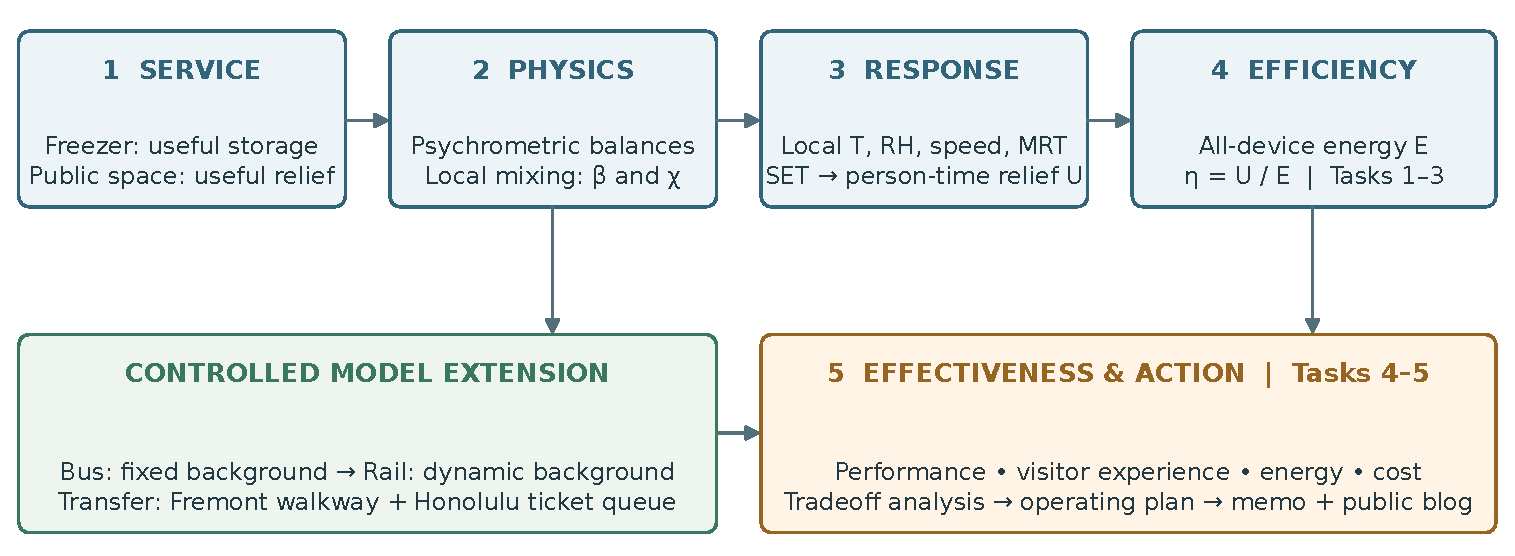
\includegraphics[width=0.82\linewidth]{figures/29_cp_set_framework.pdf}\\[-2pt]
{\small\textbf{CP-SET workflow.} One physical kernel supports progressively broader decisions.}
\end{center}
